\documentclass{beamer}
\usetheme{Madrid}
\usecolortheme{rose}

\usepackage{graphicx}
\usepackage[utf8]{inputenc}
\usepackage[T5]{fontenc}
% \usepackage[vietnamese]{babel}
\usepackage{tikz}
\usetikzlibrary{shadows}

\usepackage{amsmath}
\usepackage{amsfonts}
\usepackage{xcolor}
\usepackage{listings}
\usepackage{tcolorbox}
\setbeamertemplate{caption}{\insertcaption}
\setbeamertemplate{subsection in toc}[subsections numbered]

\tcbuselibrary{skins,breakable}
\setbeamertemplate{navigation symbols}{}
\setbeamertemplate{footline}[frame number]

\usebackgroundtemplate{
    \parbox[c][\paperheight][c]{\paperwidth}{
        
\includegraphics[width=\paperwidth,height=\paperheight]{background.jpg}
    }
}

\begin{document}

\section{Bài tập luyện tập}

\begin{frame}[plain]
    \centering
    \vspace{1cm}

    \begin{tcolorbox}[
            enhanced,
            colback=blue!70!black,
            colframe=blue!70!black,
            width=0.75\textwidth,
            arc=4mm,
            boxrule=0pt,
            drop shadow
        ]
        \centering
        {\color{white}\LARGE \textbf{Bài Tập về đồ thị}}\\[0.2cm]
        {\color{white}\large Những bài tập cơ bản nhất về dồ thị}
    \end{tcolorbox}

    \vspace{1.2cm}

    {\Large \textbf{Nguyễn Văn Phú - Hà Minh Đức - Nguyễn Tấn Đạt}}\\[0.4cm]
    THPT Chuyên ĐHV\\[0.6cm]

    March, 2026
\end{frame}

% ===== BÀI 1 =====
\begin{frame}{Bài toán 1 - Đếm thành phần liên thông}

\begin{block}{Đề bài}
Cho một đồ thị vô hướng gồm $n$ đỉnh và $m$ cạnh.  
Hãy đếm số \textbf{thành phần liên thông}.
\end{block}

\pause

\begin{alertblock}{Gợi ý}
Sử dụng DFS hoặc BFS để duyệt từng thành phần.
\end{alertblock}

\pause

\begin{center}
\textbf{Chi tiết bài tập:}

\vspace{0.3cm}

\href{https://codeforces.com/problemset/problem/166/A}{\color{blue}{Click vào đây}}
\end{center}

\end{frame}

% ===== SOLUTION 1 =====
\begin{frame}[fragile]{Solution - Bài 1}

\begin{block}{Ý tưởng}
\begin{itemize}
    \item Duyệt qua từng đỉnh
    \item Nếu đỉnh chưa thăm → chạy DFS/BFS
    \item Mỗi lần chạy → tăng số thành phần lên 1
\end{itemize}
\end{block}

\pause

\begin{tcolorbox}[colback=black!5!white,colframe=blue!75!black,title=Mã giả DFS]
\begin{verbatim}
for u in V:
    if not visited[u]:
        DFS(u)
        count += 1
\end{verbatim}
\end{tcolorbox}

\end{frame}

% ===== BÀI 2 =====
\begin{frame}{Bài toán 2 - Đường đi ngắn nhất}

\begin{block}{Đề bài}
Cho đồ thị không trọng số.  
Tìm khoảng cách ngắn nhất từ đỉnh $s$ đến tất cả các đỉnh còn lại.
\end{block}

\pause

\begin{alertblock}{Gợi ý}
Sử dụng BFS để đảm bảo đi theo từng lớp.
\end{alertblock}

\pause

\begin{center}
\textbf{Chi tiết bài toán:}

\vspace{0.3cm}

\href{https://codeforces.com/problemset/problem/20/C}{\color{blue}{Click để thử sức}}
\end{center}

\end{frame}

% ===== SOLUTION 2 =====
\begin{frame}[fragile]{Solution - Bài 2}

\begin{block}{Ý tưởng}
\begin{itemize}
    \item Khởi tạo khoảng cách $dist[s] = 0$
    \item Dùng queue để BFS
    \item Mỗi lần đi qua cạnh → cập nhật khoảng cách
\end{itemize}
\end{block}


\end{frame}

\begin{frame}
    \begin{exampleblock}{Mã giả BFS}
        \begin{center}
            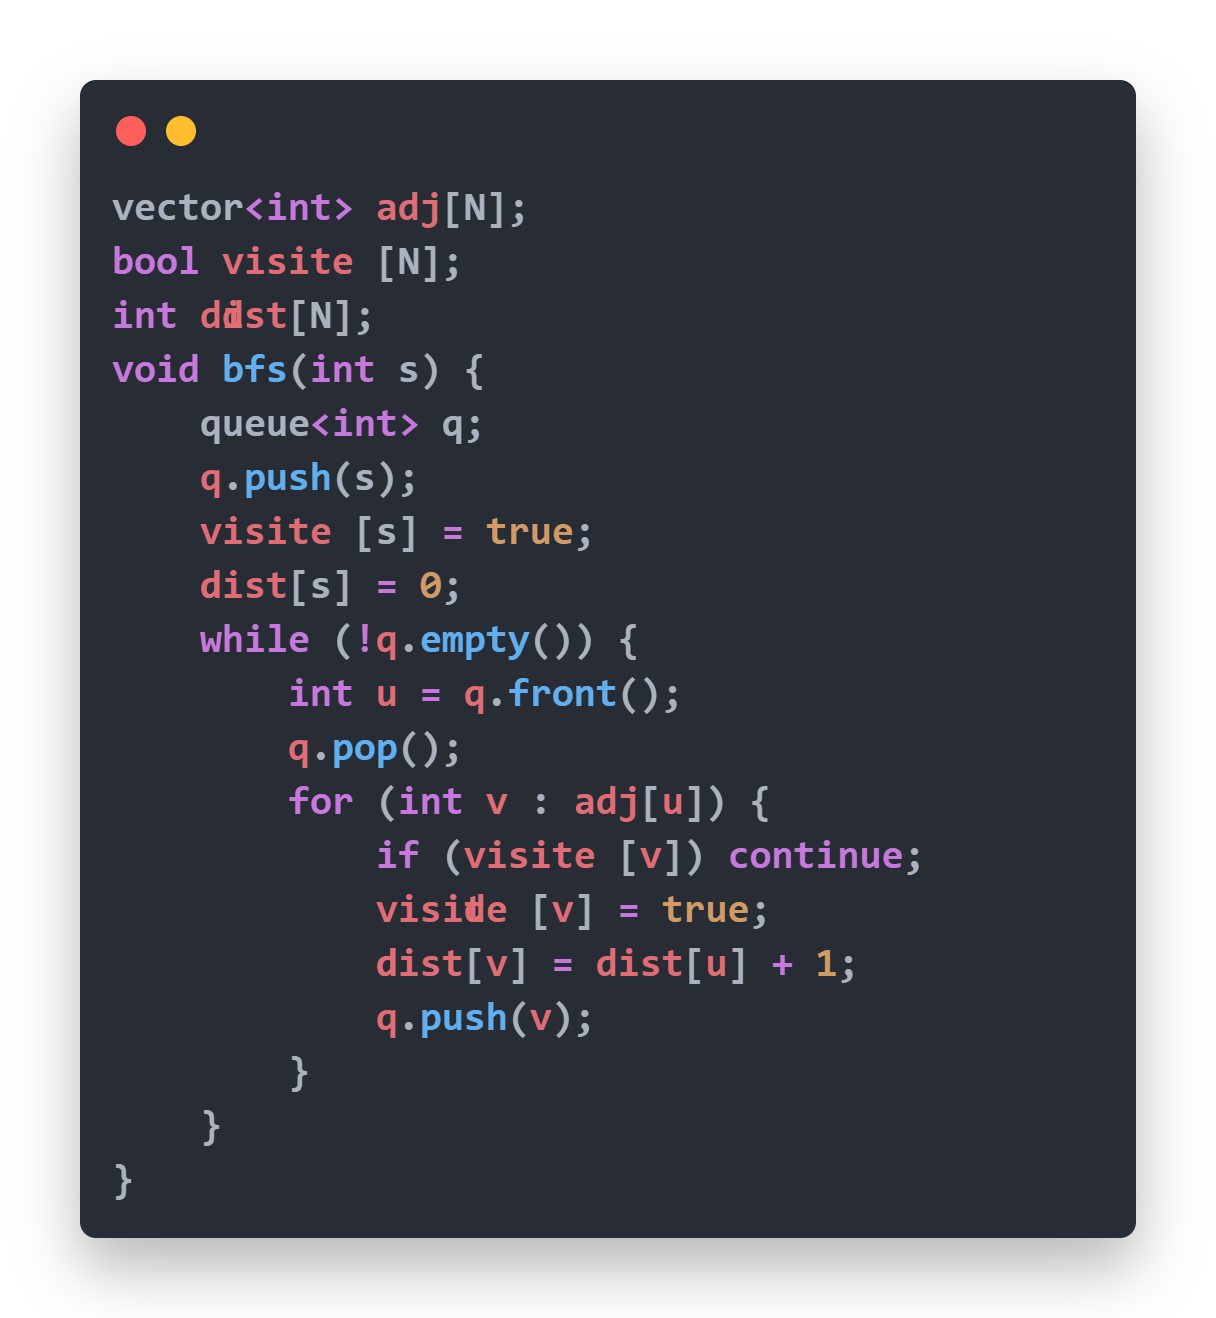
\includegraphics[width=0.6\textwidth]{codemau1.png}
        \end{center}
    \end{exampleblock}
    
\end{frame}

% ===== BÀI 3 =====
\begin{frame}{Bài toán 3 - Phát hiện chu trình}

\begin{block}{Đề bài}
Cho đồ thị vô hướng.  
Kiểm tra xem đồ thị có chứa chu trình hay không.
\end{block}

\pause

\begin{alertblock}{Gợi ý}
Dùng DFS và lưu đỉnh cha.
\end{alertblock}

\pause

\begin{center}
\textbf{Link luyện tập:}

\vspace{0.3cm}

\href{https://cses.fi/problemset/task/1669}{\color{blue}{Cycle Detection - CSES}}
\end{center}

\end{frame}

% ===== SOLUTION 3 =====
\begin{frame}[fragile]{Solution - Bài 3}

\begin{block}{Ý tưởng}
\begin{itemize}
    \item Khi DFS từ $u$ sang $v$
    \item Nếu $v$ đã thăm và $v \neq parent[u]$ → có chu trình
\end{itemize}
\end{block}

\pause

\begin{tcolorbox}[colback=black!5!white,colframe=red!70!black,title=Mã giả DFS]
\begin{verbatim}
DFS(u, parent):
    visited[u] = true
    for v in adj[u]:
        if not visited[v]:
            if DFS(v, u): return true
        else if v != parent:
            return true
    return false
\end{verbatim}
\end{tcolorbox}

\end{frame}

% ===== SLIDE TỔNG KẾT =====
\begin{frame}{Tổng kết luyện tập}

\begin{block}{Những dạng quan trọng}
\begin{itemize}
    \item DFS → thành phần liên thông, chu trình
    \item BFS → đường đi ngắn nhất
    \item Kết hợp → nhiều bài nâng cao
\end{itemize}
\end{block}

\pause

\begin{center}
\Huge  \textcolor{orange}{Practice makes perfect!}
\end{center}

\end{frame}

\end{document}
